\subsubsection{Design of Instruction Set} \label{sec:design-instruction-set}

OlaVM utilizes the Reduced Instruction Set Computer (RISC) architecture, which is characterized by a smaller instruction set 
compared to the Complex Instruction Set Computer (CISC) architecture.
The contrast between RISC and CISC architectures can be further explored in the \href{https://cs.stanford.edu/people/eroberts/courses/soco/projects/risc/risccisc/}{RISC vs. CISC comparison}.

\emph{1. A reduced instruction set reduces the number of constraint polynomials}

In ZKVM, there is a very critical constraint, the CSTC (CPU State Transition Constraint); it is mainly used to constrain the validity
of VM state changes before and after the execution of an instruction.

\begin{figure}[!ht]
    \centering
    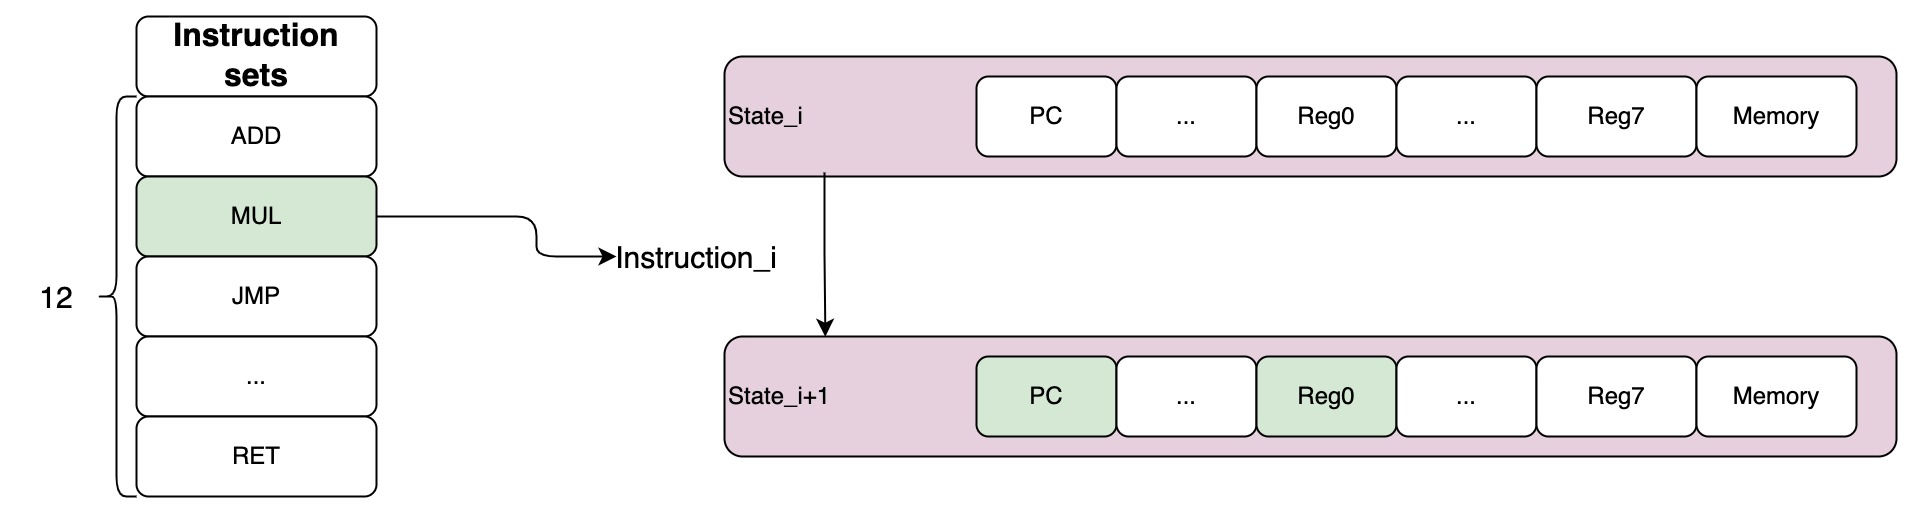
\includegraphics[width=0.7\textwidth]{vm/olavm-instruction-state.jpeg}
    \caption{Instruction-induced cpu state transition}
    \label{fig:instruction-cpu-state-transition}
\end{figure}

As shown in \figref{fig:instruction-cpu-state-transition}, there are many registers in the VM. When the VM executes an instruction, it will
cause the state of some registers to change, in order to ensure the correctness of the VM execution, we need to constrain the following:
\begin{itemize}
    \item The change of register state involved in the execution of the instruction is valid;
    \item The status of registers not involved in the instruction execution remains unchanged.
\end{itemize}

Let's look at a simple example to explain the constraints on register state changes:
\begin{table}[!ht]
    \centering
    \begin{tabular}{|c|c|c|c|c|c|c|c|}
        \hline
        \rowcolor{gray} clk & pc    & instruction        & \dots & reg0  & reg1  & reg2  & \dots \\
        \hline
        \dots               & \dots & \dots              & \dots & \dots & \dots & \dots & \dots \\
        \hline
        78                  & 8     & ADD reg0 reg0 reg1 & \dots & 1     & 2     & 0     & \dots \\
        \hline
        79                  & 9     & MOV reg2 3         & \dots & 3     & 0     & 0     & \dots \\
        \hline
        80                  & 11    & JMP 2              & \dots & 3     & 0     & 3     & \dots \\
        \hline
        81                  & 2     & \dots              & ...   & 3     & 0     & 3     & \dots \\
        \hline
    \end{tabular}
    \caption{Example of cpu state transitions}
    \label{table:example-cpu-state-transitions}
\end{table}

\tabref{table:example-cpu-state-transitions} briefly presents the changes of some registers after the VM executes three
instructions; taking the PC register as an example, the logic of the updates of the three instructions are:
\begin{itemize}
    \item ADD: $\mathrm{pc}_{i+1} = \mathrm{pc}_i + 1$
    \item MOV: $\mathrm{pc}_{i+1} = \mathrm{pc}_i + 2$
    \item JMP: $\mathrm{pc}_{i+1} = 2$
\end{itemize}

When considering constraints, we cannot predict which instruction the VM will execute at any given time. 
Therefore, we must design a constraint capable of handling all instructions. This constraint is known as the CPU State Transition Constraint (CSTC). 
In the aforementioned simple example, the update logic of the PC can be designed as follows:
\[ \mathrm{pc}_{i+1} = \mathrm{sel\_jmp}_i \cdot \mathrm{imm\_value} + (1 - \mathrm{sel\_jmp}) \cdot (\mathrm{pc}_i + 1 + \mathrm{op1\_imm}) \]

We express all CPU state transitions in this constrained form. The inclusion of each new instruction introduces additional selectors, which increases the complexity of the constraints. 
To manage this complexity, we limit the instruction size to 19, including built-ins.

Despite having a reduced instruction set architecture, it is still necessary to maintain Turing-completeness to ensure that we can perform any computation with these simple instructions. 
Combining these instructions with the prophet mechanism described in Section \ref{sec:design-prophet}, we have developed Ola-lang, a Turing-complete language that supports loops and recursive operations.


\emph{2. Most of the operations will use a small part of the instruction set}

Under the CISC architecture, a vast instruction set is defined. However, in practice, only a small subset of the instructions is used for most computations. From a constraint standpoint, this represents a significant inefficiency. 
This is because the constraint logic for all instructions must be included in the constraint system (CSTC), and in the worst-case scenario, each instruction corresponds to a constraint factor. 
This complexity can lead to a large number of polynomials and high-order constraints, making the entire constraint system challenging to scale.

\begin{figure}[!ht]
    \centering
    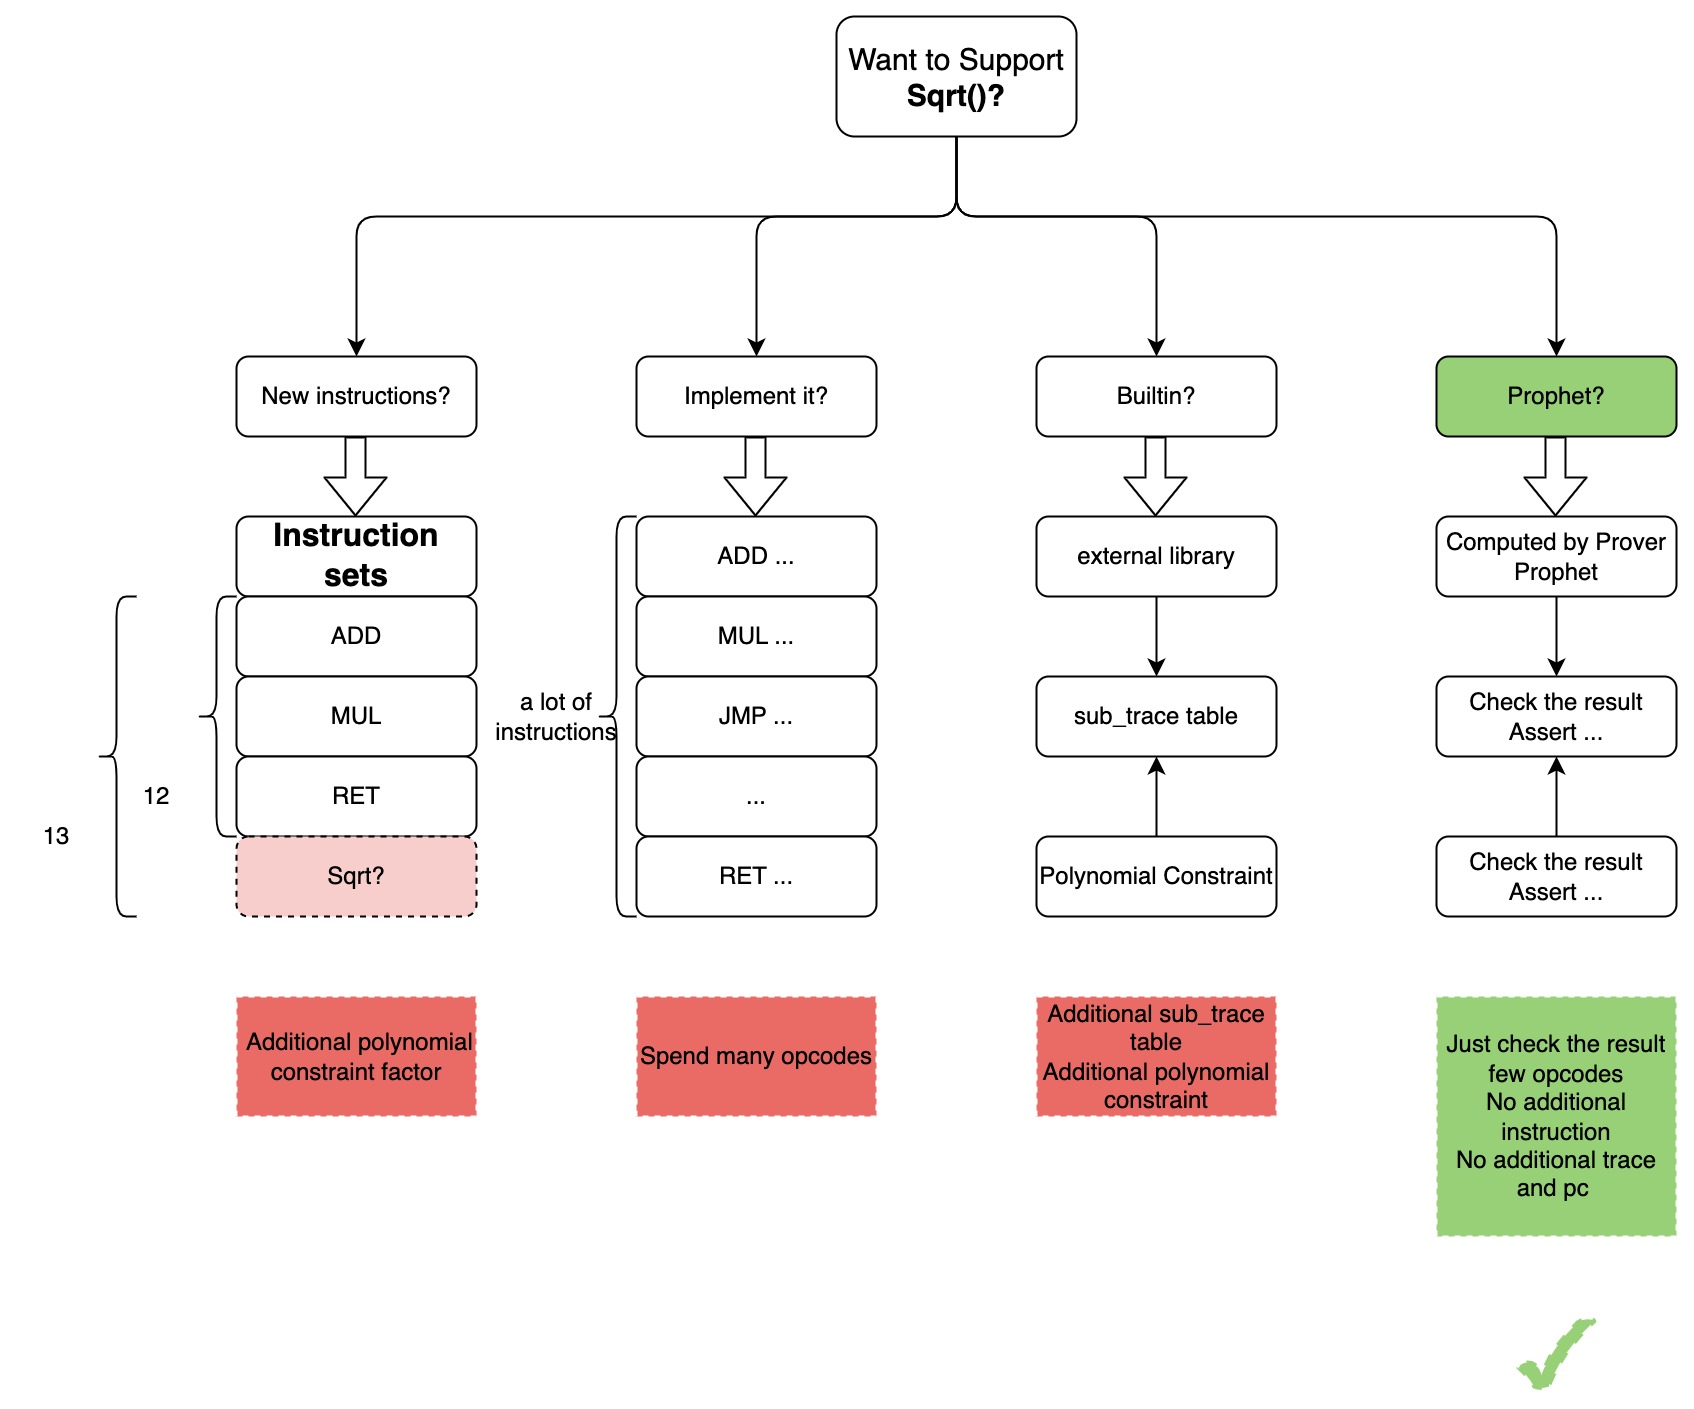
\includegraphics[width=0.6\textwidth]{vm/design-support-zk-unfriendly.jpeg}
    \caption{The best way to support ZK-Unfriendly computation}
    \label{fig:desgin-support-zk-unfriendly}
\end{figure}

In many cases, when performing certain calculations, it is preferable to use the existing instruction set instead of introducing a new instruction.
While this approach may increase the program size (in terms of opcodes), redundant data can be added during the verification process to facilitate FFT. 
However, for complex computations that require a significant number of instructions, other solutions are available. These include introducing Builtins and our Prophet module, which will be discussed in more detail in subsequent chapters. 
For now, it is important to note that they can significantly reduce the number of instructions needed to perform these complex computations, as demonstrated in \figref{fig:desgin-support-zk-unfriendly}.